\chapter{Experiment}

This chapter primarily discusses the trajectory performance of the robot in different test scenarios, detailing the parameters of both the controller and the robot. Additionally, this chapter provides a brief evaluation of the accuracy and applicability of the SMC controller under various test conditions.

\section{Experimental Setup}

In this section, we outline the relevant parameters and simulation environment used in the experiment:
\begin{itemize}
    \item \textbf{Vehicle Parameters}: Provide details about the simulated vehicle model, including maximum speed(), maximum angular velocity, turning radius, initial coordinates, and initial angle.

    \item \textbf{SMC Parameters}: List the key parameters for the SMC controller, such as the control gain \( \gamma \), boundary distance \( d_{\text{safe}} \), and switching thresholds \( \delta \).
    \item \textbf{Simulation Environment}: Describe the simulation tools (e.g., MATLAB) and settings, including grid size, time steps, and visualization setup.
\end{itemize}

\section{Testing Scenarios}

Each of the following test scenarios represents a different type of environment to evaluate the SMC controller's effectiveness in navigation tasks.

\subsection{Simulation of Static Obstacles Avoidance}
In this scenario, stationary point obstacles are placed at fixed coordinates \((1, 1)\), \((2, 2)\), and \((3, 3)\) within a bounded simulation environment. The mobile robot is initialized at the origin \((0, 0)\) with a heading angle of \(0\), facing the positive \(x\)-axis. The obstacles are modeled as point objects with no dynamic behavior, allowing the robot to focus solely on path planning and avoidance using the sliding mode control algorithm.

The simulation parameters are set as follows: the robot maintains a constant linear velocity of \(1\,\text{m/s}\) and adjusts its angular velocity based on the sliding mode control law, with a maximum angular velocity \(u_{\text{max}} = 1.5\,\text{rad/s}\). The safety distance \(d_{\text{safe}} = 2\,\text{m}\) ensures the robot remains sufficiently clear of obstacles throughout the trajectory. The controller parameters \(\gamma = 2\) and \(\delta = 2\) are chosen to balance the responsiveness and stability of the sliding mode control, while \(v_\ast = \gamma \cdot \delta = 4\) defines the maximum adjustment for \(\chi(z)\) in the nonlinear control region.

The robot navigates the environment by continuously monitoring the distance \(d(t)\) to the closest obstacle and computing the rate of change of distance \(\dot{d}(t)\) using numerical differentiation. The sliding mode control law governs the angular velocity \(u(t)\) as:
\begin{equation}
u(t) = u_{\text{max}} \cdot \text{sign} \left( \dot{d}(t) + \chi[z(t)] \right),
\end{equation}
where \(z(t) = d(t) - d_{\text{safe}}\) and the auxiliary function \(\chi(z)\) is defined as:
\begin{equation}
\chi(z) =
\begin{cases}
\gamma \cdot z, & \text{if } |z| \leq \delta, \\
v_\ast \cdot \text{sign}(z), & \text{if } |z| > \delta.
\end{cases}
\end{equation}

During the course of \(200\) simulation steps (\(20\,\text{s}\) total simulation time, with a time step of \(0.1\,\text{s}\)), the robot's trajectory is recorded and analyzed. The results demonstrate the robot's ability to successfully navigate the environment while maintaining a safe distance from all obstacles. The trajectory is visualized in Figure \ref{FIG:2}, where the robot's path is represented by a red line, and obstacles at stationary points are marked as red "×" symbols.

\begin{figure}[H]
    \centering
    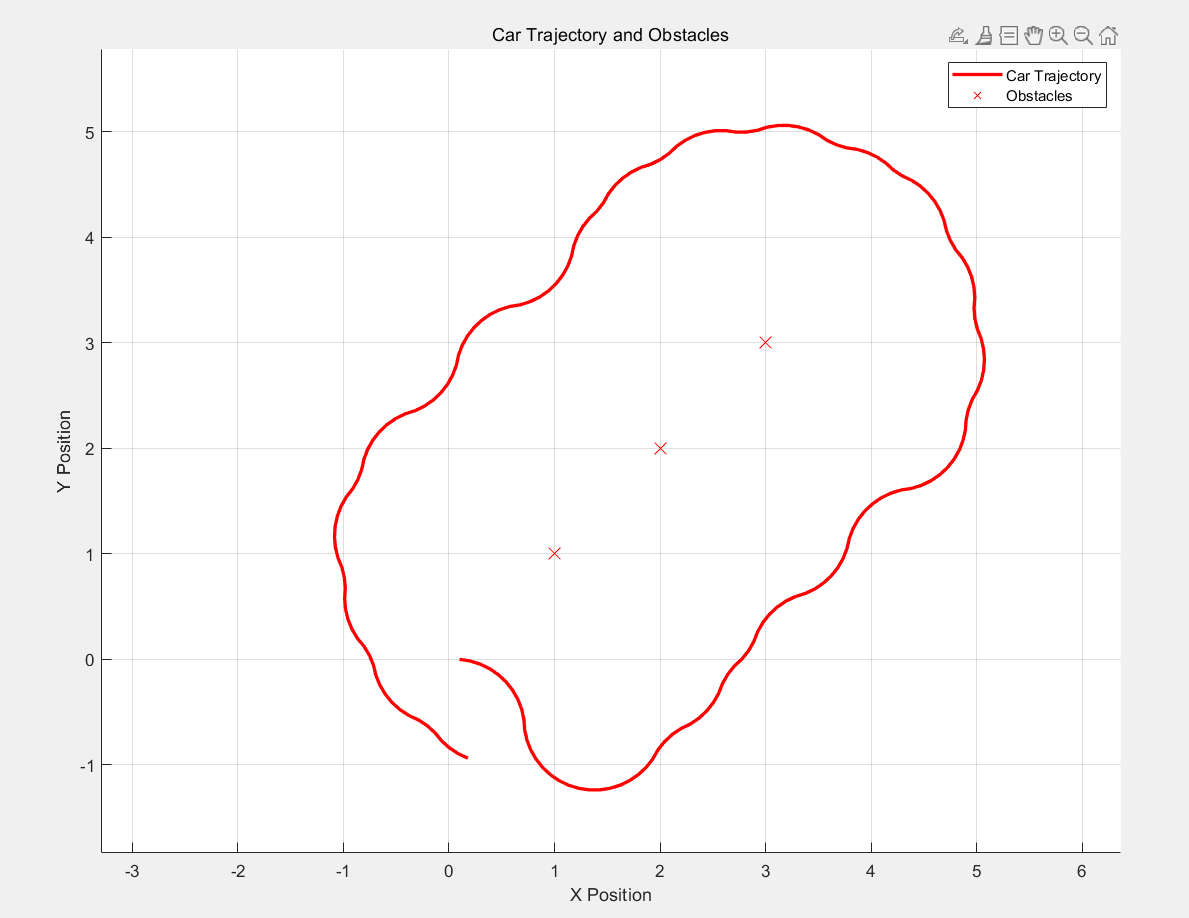
\includegraphics[scale=0.5]{2.png}
    \caption{Car Trajectory} % 图名称
    \label{FIG:2}
\end{figure}

The temporal evolution of the distances between the robot and each obstacle is illustrated in Figure \ref{FIG:3}. Each curve corresponds to a specific obstacle, showing how the robot dynamically adjusts its trajectory to maintain a safe distance. At the start of the simulation, the robot rapidly approaches the nearest obstacle, causing the corresponding distance curve to decrease. Once the robot reaches the minimum allowable distance (\(d_{\text{safe}} = 2 \, \text{m}\)), the sliding mode controller adjusts its motion to maintain the safety threshold while maneuvering around the obstacle.

\begin{figure}[H]
    \centering
    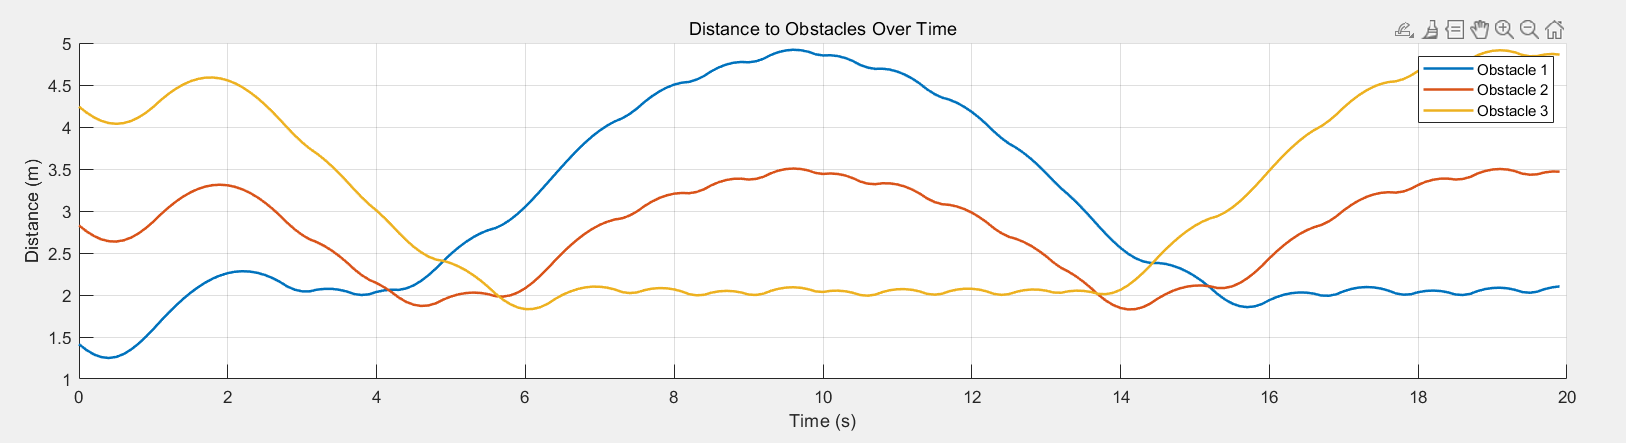
\includegraphics[width=0.8\textwidth]{3.png}
    \caption{Robot-Obstacle Distance Profiles}
    \label{FIG:3}
\end{figure}

Based on the distance graph in Figure~\ref{FIG:3}, it can be observed that the curve exhibits irregular oscillations, reflecting the robot's dynamic adjustments (sgn function) as it transitions between the influence regions of multiple obstacles. This also demonstrates the real-time responsiveness of the sliding mode control algorithm. Notably, the distance curve rarely falls below the predefined safety threshold. For instance, as shown in the figure, the orange curve remains above the set safety threshold while approaching Obstacle 3 during the 6-14 time units.

This analysis supports the effectiveness of the SMC control algorithm in maintaining safe navigation in environments with multiple static obstacles.



\subsection{Simulation of Moving Obstacles Avoidance}


\subsubsection{Initial Setup and Motion Description}


To investigate the obstacle avoidance performance of the Sliding Mode Control (SMC) algorithm under dynamic obstacles, four moving obstacles are introduced in this environment.

\begin{itemize}
    \item \textbf{Ob1}: Initial position \((2, 2)\), moving with velocity \((0.1, 0)\) m/s.
    \item \textbf{Ob2}: Initial position \((1, 2)\), moving with velocity \((-0.1, 0.1)\) m/s.
    \item \textbf{Ob3}: Initial position \((3, 3)\), moving with velocity \((0.1, -0.1)\) m/s.
    \item \textbf{Ob4}: Initial position \((4, 4)\), moving with velocity \((0.2, 0.1)\) m/s.
\end{itemize}

Detailed information about the obstacles and the initial position of the robot can be found in Figure~\ref{FIG:4}. In the figure, the robot's initial position is represented by a green circle, and the direction of motion for each obstacle is indicated with arrows.

\begin{figure}[H]
    \centering
    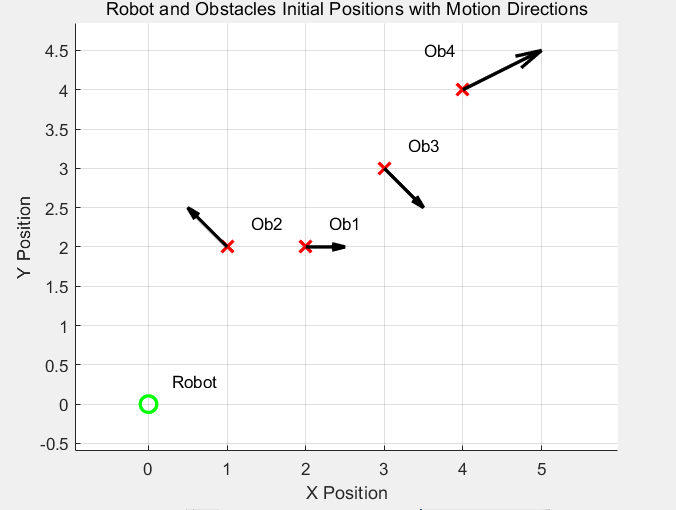
\includegraphics[width=0.8\textwidth]{4.png}
    \caption{Initial Positions and Motion Directions of Robot and Obstacles}
    \label{FIG:4}
\end{figure}

\subsubsection{Robot and Obstacle Trajectories}

The robot's trajectory under sliding mode control is depicted in Figure \ref{FIG:5} alongside the moving trajectories of the obstacles. The robot dynamically adjusts its heading to maintain a safe distance from obstacles, as defined by the \(d_{\text{safe}}\) parameter. It can be observed that the SMC algorithm effectively guides the robot through the environment, successfully avoiding collisions while navigating between the moving obstacles. This figure demonstrates the robot's adaptability to changes in obstacle positions and motion patterns.

\begin{figure}[H]
    \centering
    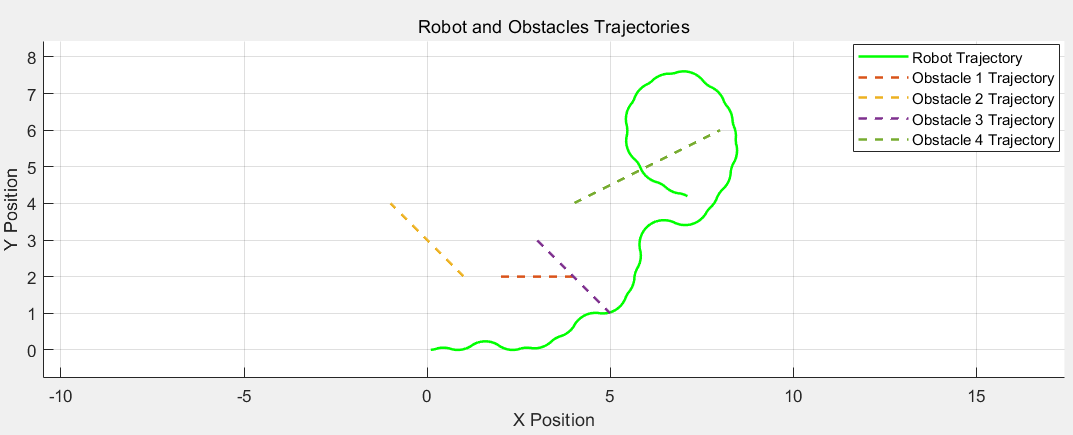
\includegraphics[width=0.8\textwidth]{5.png}
    \caption{Robot and Obstacles Trajectories}
    \label{FIG:5}
\end{figure}

\subsubsection{Temporal Evolution of Distances}

The robot-obstacle distance profiles over the 20-second simulation period are shown in Figure \ref{FIG:6}. Each curve corresponds to a specific obstacle, highlighting the robot's ability to maintain a minimum safety distance of \(2\,\text{m}\) throughout the test. The oscillatory patterns in the distance profiles reflect the robot's real-time responses to obstacle movements and interactions with multiple obstacles.

\begin{figure}[H]
    \centering
    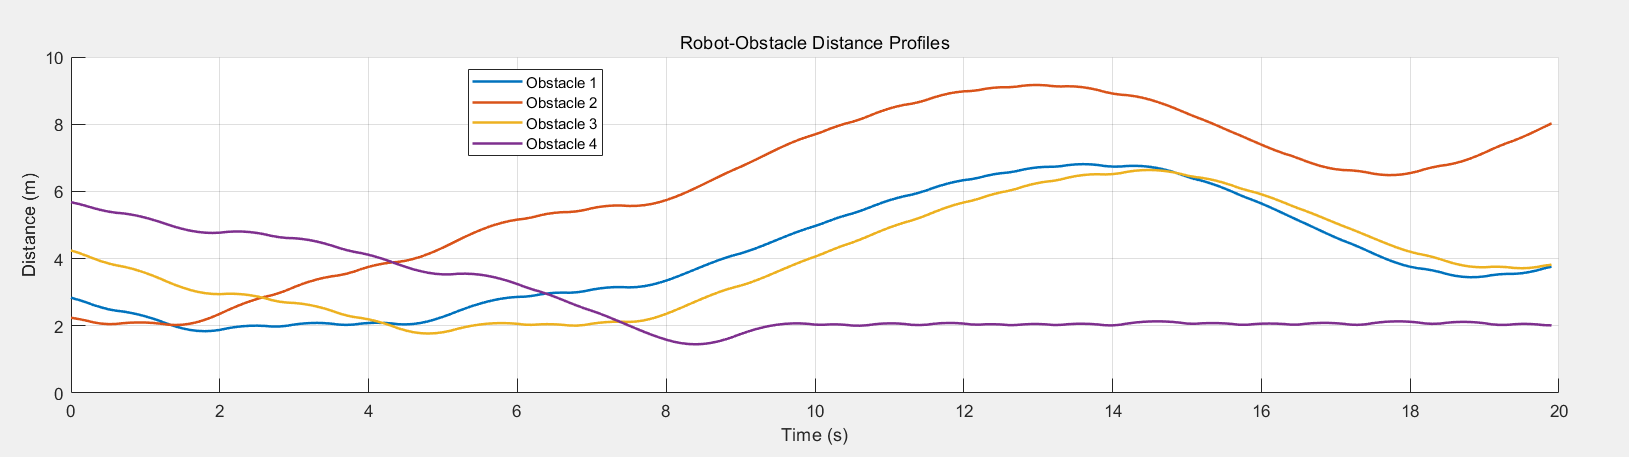
\includegraphics[width=0.8\textwidth]{6.png}
    \caption{Temporal Evolution of Robot-Obstacle Distances}
    \label{FIG:6}
\end{figure}

\subsubsection{Discussion}

The results validate the robustness of the SMC algorithm in environments with dynamic obstacles. The robot's trajectory demonstrates smooth transitions and efficient avoidance maneuvers, while the distance profiles confirm the maintenance of the safety threshold. This test highlights the capability of SMC to handle more complex and dynamic environments, laying the groundwork for future applications in real-world scenarios.

\subsection{Navigation to Target in a Static Obstacle Field}

In this test scenario, the initial position of the robot is set at $(0, 0)$, and the target point is located at $(5, 4)$. The environment contains three static obstacles with coordinates $(1, 1)$, $(2, 2)$, and $(4, 3)$, respectively. During path planning, the robot must navigate around the obstacles while maintaining a safety distance of $d_{\text{safe}} = 2$ and eventually reach the target point.

As shown in Figure \ref{FIG:7}, the green trajectory line represents the actual path taken by the robot, the red crosses indicate the positions of the obstacles, and the blue circle denotes the target point. The dashed circles are centered on the obstacles, with a radius equal to the adjusted triggering distance $d_{\text{safe}} - \varepsilon$. These dashed circles represent the influence zones of the obstacles. When the robot enters these zones, it activates the obstacle avoidance mode, adjusting its angular velocity $u$ using sliding mode control to change direction and avoid collisions. Once the robot exits these zones, it switches to the target-following mode, moving directly toward the target point.
\begin{figure}[H]
    \centering
    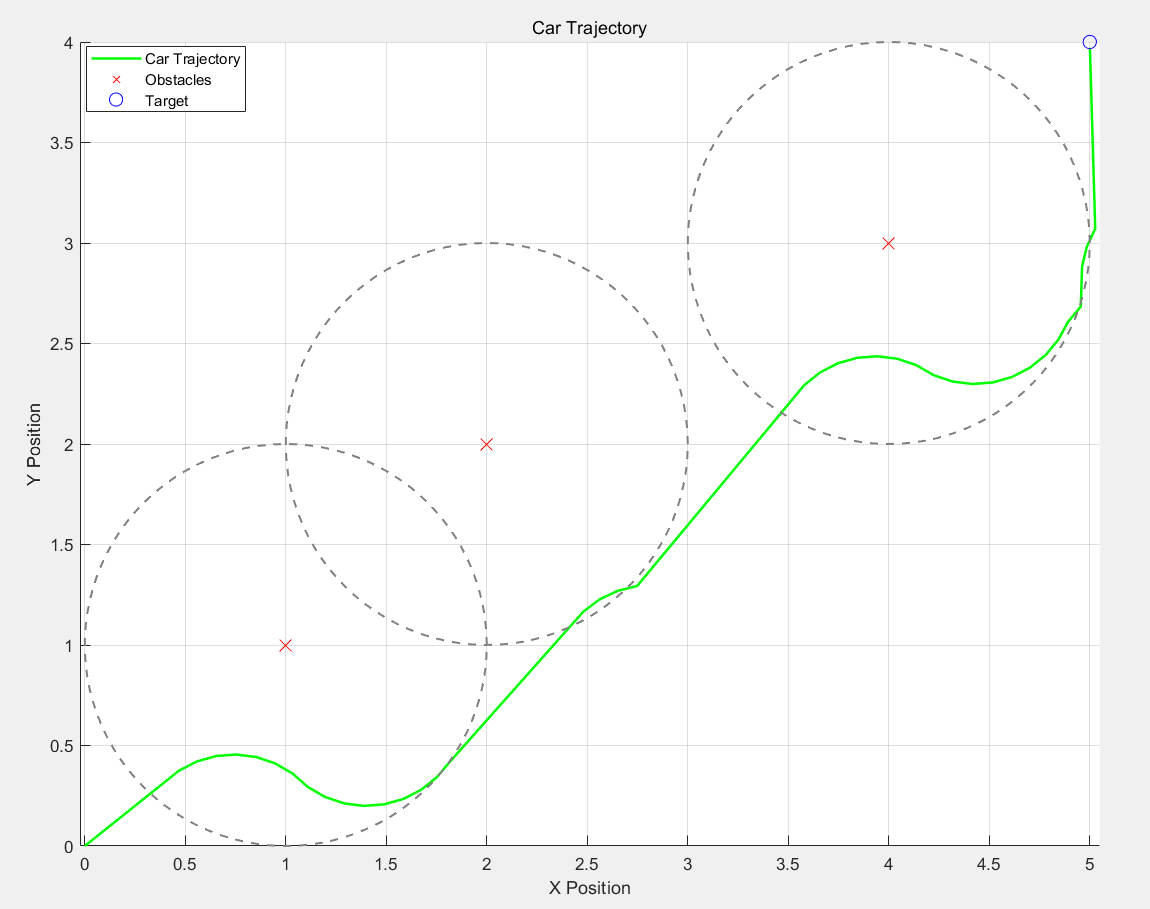
\includegraphics[width=0.8\textwidth]{7.png}
    \caption{Car Trajectory}
    \label{FIG:7}
\end{figure}

It is important to note that the obstacle avoidance and target-following mode switching logic implemented in this experiment is based on the goal-seeking algorithm proposed in Section 7 of the Reference \cite{Matveev2012}. 

The switching between the Proposed Guidance Law (PGL) and the Velocity Obstacle Approach (VOA)\cite{Fiorini1998} is the core logic for enabling the robot to navigate smoothly to the target. When the robot detects the nearest obstacle within a certain range, it calculates the distance $d_t$ to the closest obstacle and compares it to the threshold triggering distance $d_{\text{safe}} - \varepsilon$. Here, $d_{\text{safe}}$ represents the predefined safety distance, and $\varepsilon$ is an adjustable parameter that fine-tunes the triggering condition. Once $d_t \leq d_{\text{safe}} - \varepsilon$, the robot activates obstacle avoidance mode, during which sliding mode control is employed to regulate the robot's angular velocity $u$.

Sliding mode control uses the deviation $z = d_t - d_{\text{safe}}$ to compute the control law. If $|z| > \delta$, a proportional control $\chi_z = v^* \cdot \text{sign}(z)$ is applied to ensure rapid adjustments, where $v^*$ is the switching velocity determined by the algorithm parameters. Conversely, when $|z| \leq \delta$, a linear control $\chi_z = \gamma \cdot z$ is used, where $\gamma$ represents a constant gain. This hybrid control strategy ensures that the robot avoids obstacles efficiently while minimizing abrupt changes in direction.

When the robot exits the obstacle's influence zone, such that $d_t > d_{\text{safe}} - \varepsilon$, it switches to the target-following mode. In this mode, the robot calculates the direction angle $\theta_{\text{to target}}$ toward the target and moves along a straight line with a constant linear velocity $v$, aligning its heading angle $\theta$ with $\theta_{\text{to target}}$.

In practical operation, this algorithm demonstrates its efficiency in complex environments. By appropriately tuning the parameter $\varepsilon$, it achieves optimal path planning while avoiding obstacles, validating the applicability and effectiveness of the reference algorithm in scenarios with static obstacles.


\subsection{Navigation to Target in a Moving Obstacle Field}

This section will test the ability of the wheeled robot to avoid multiple moving obstacles and navigate to the target using the sliding mode control method. The settings for this scenario are as follows: the robot starts from an initial position of $(0, 0)$ and aims to reach a target located at $(3, 4)$, represented by a red hollow circle. The trajectory of the robot is shown in the figure \ref{FIG:8}.

\begin{figure}[H]
    \centering
    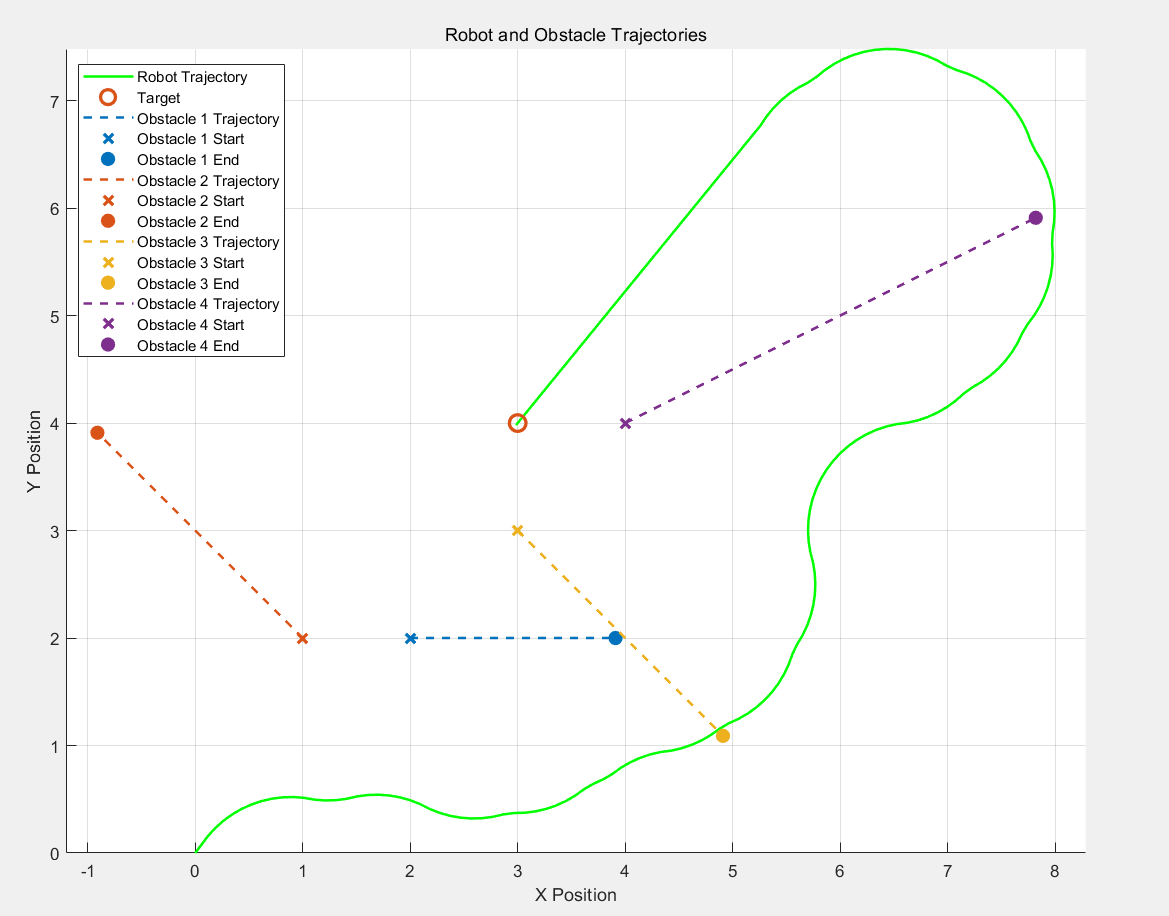
\includegraphics[width=0.8\textwidth]{8.png}
    \caption{Robot and Obstacles Trajectories}
    \label{FIG:8}
\end{figure}

\subsubsection{Parameter Settings}

The simulation parameters include a time step of $\Delta t = 0.1$ and a maximum simulation time of $t_{\text{max}} = 20$. The robot linear velocity is set to $v = 1.0$, with a maximum angular velocity of $u_{\text{max}} = 1.0$. For collision avoidance, a safe distance of $d_{\text{safe}} = 2.0$ is used. The sliding mode control parameters are $\gamma = 0.4$ and $\delta = 0.7$, and the proximity threshold to determine the target reach is $0.05$. 

The dynamic obstacles are initialized with specific properties, including their initial positions and velocities, as well as their trajectories, which are visualized in Figure 4.8. The initial positions and velocities are as follows: Obstacle 1 starts at position \((2.0, 2.0)\) with velocity \((0.1, 0.0)\), Obstacle 2 starts at position \((1.0, 2.0)\) with velocity \((-0.1, 0.1)\), Obstacle 3 starts at position \((3.0, 3.0)\) with velocity \((0.1, -0.1)\), and Obstacle 4 starts at position \((4.0, 4.0)\) with velocity \((0.2, 0.1)\). The trajectories of these obstacles, including their start and end points, are recorded as follows: Obstacle 1 travels from \((2.0, 2.0)\) to \((0.0, 2.0)\), Obstacle 2 from \((1.0, 2.0)\) to \((1.0, 4.0)\), Obstacle 3 from \((3.0, 3.0)\) to \((2.0, 2.0)\), and Obstacle 4 from \((4.0, 4.0)\) to \((6.0, 6.0)\).

\begin{figure}[H]
    \centering
    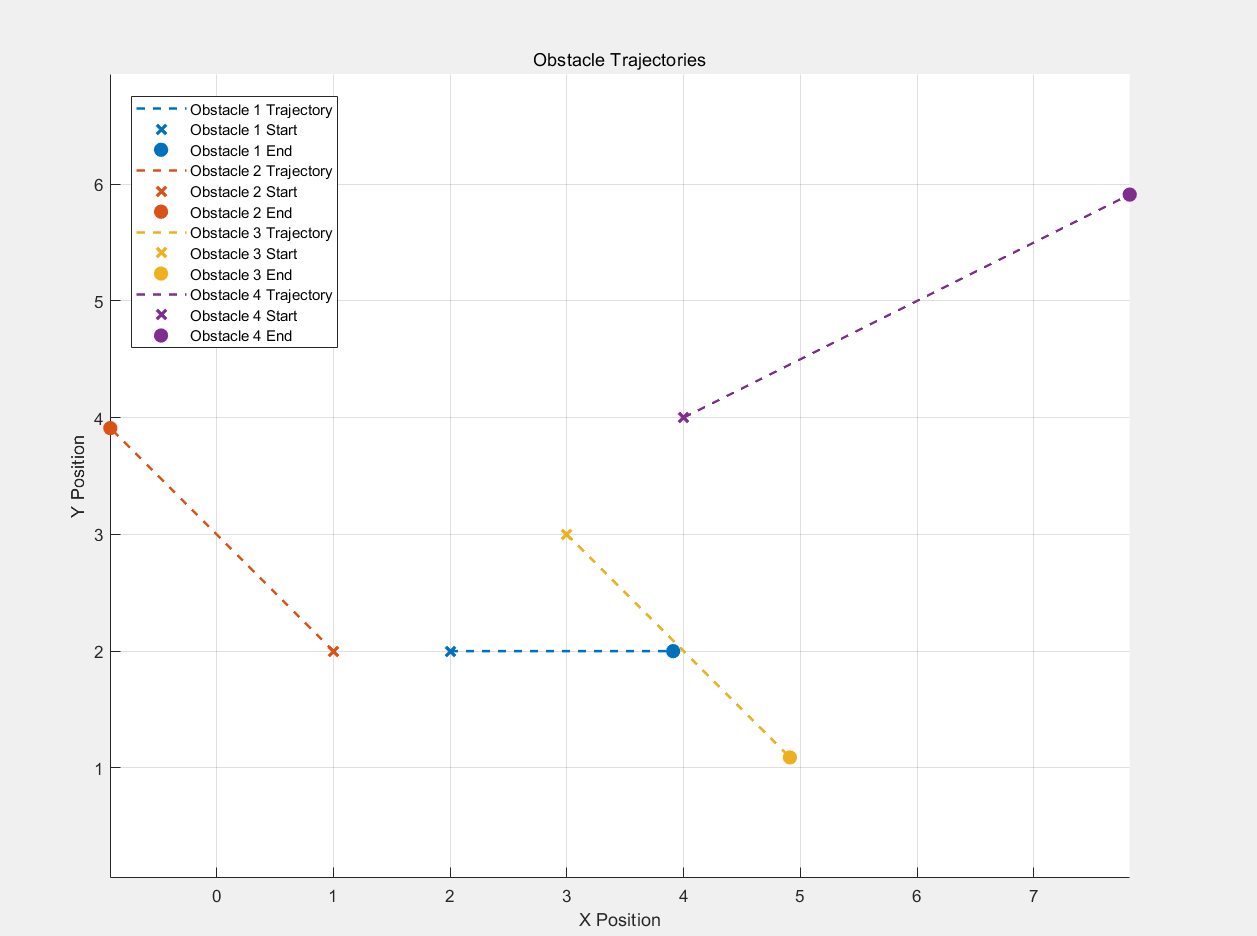
\includegraphics[width=0.8\textwidth]{9.png}
    \caption{Obstacles Trajectory}
    \label{FIG:9}
\end{figure}

\subsubsection{Simulation Results and Trajectory Analysis}

The robot's trajectory and obstacle avoidance behavior are analyzed in Figure~\ref{FIG:10}. When obstacles are distant from the robot, it moves directly toward the target along a straight line. However, as obstacles approach the safe distance threshold ($d_t \leq d_{\text{safe}}$), the robot's trajectory smoothly deviates to avoid collisions, showcasing the dynamic adjustments facilitated by the sliding mode control strategy. 


\begin{figure}[H]
    \centering
    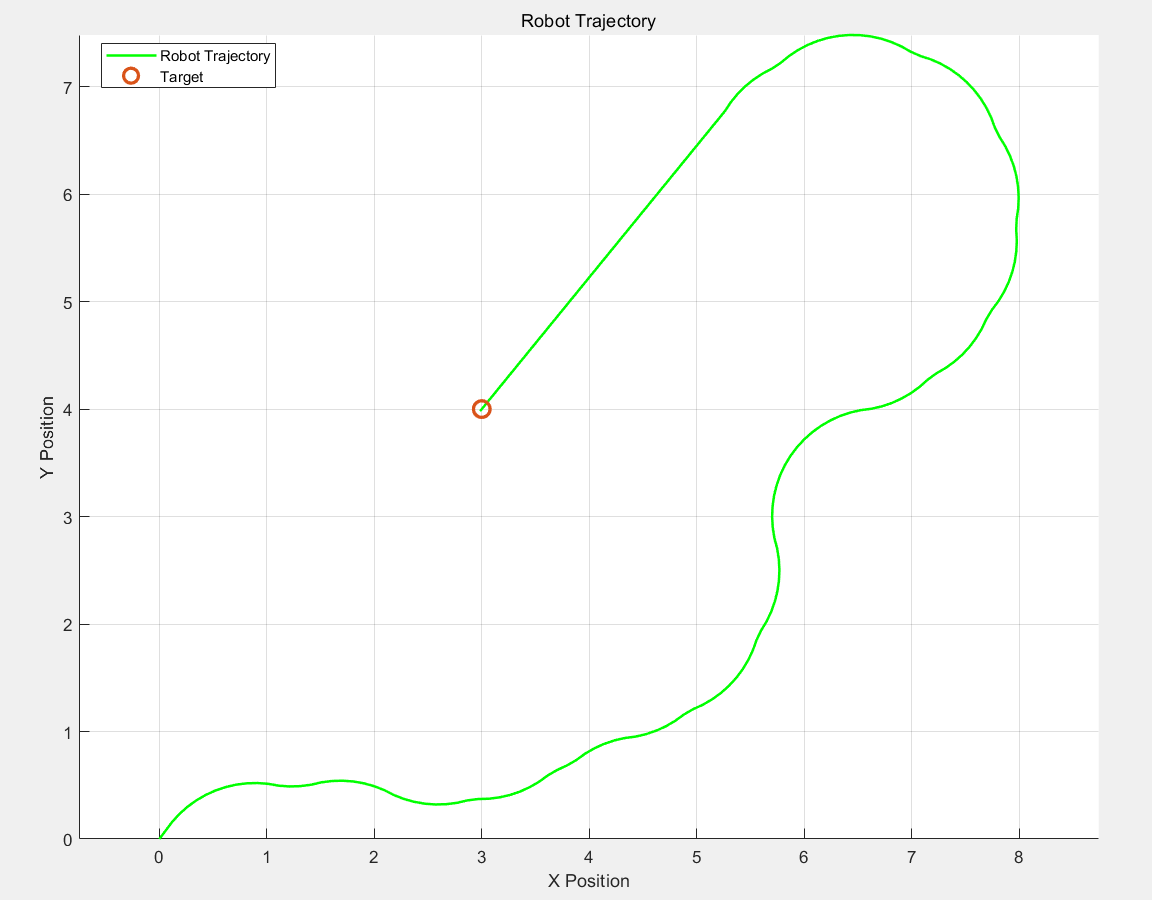
\includegraphics[width=0.8\textwidth]{10.png}
    \caption{Robot Trajectory}
    \label{FIG:10}
\end{figure}

The obstacle trajectories are visualized as dashed lines, with start and end points marked by “$\times$” and solid circles, respectively. For example, obstacle 2 exhibits vertical motion, while obstacle 4 moves diagonally away. These trajectory patterns confirm the accuracy of the initial velocity settings.
In the test scenario where the robot advances toward the target in the presence of dynamic obstacles, additional parameters need to be introduced to control the robot's trajectory to prevent collisions with unpredictable dynamic obstacles. The consideration of specific parameters refers to a series of inequalities mentioned in \cite{Matveev2012}. Next, I will list these inequality requirements one by one and calculate the relevant parameters for this scenario based on these formulas.

\subsubsection*{Parameter Selection and Calculation}

In the navigation and obstacle avoidance strategy, the parameters \(\varepsilon\), \(d_0\), and \(C\) must satisfy specific constraints to ensure system feasibility and safety. Additionally, the dynamic range of obstacles \(\mathcal{R}_{\text{max}}^{\text{av}}\), the robot’s turning radius \(R\), and the minimum obstacle distance \(d_{\text{obs}}\) are calculated to define these constraints. 

The dynamic range of obstacles is calculated as:
\begin{equation}
\mathcal{R}_{\text{max}}^{\text{av}} = \sqrt{(v_x \cdot t_{\text{max}})^2 + (v_y \cdot t_{\text{max}})^2},
\end{equation}
resulting in a maximum value of \(\mathcal{R}_{\text{max}}^{\text{av}} = 4.472\). The robot’s turning radius is determined as:
\begin{equation}
R = \frac{v}{u_{\text{max}}} = 0.5,
\end{equation}
and the minimum obstacle distance is constrained by:
\begin{equation}
d_{\text{obs}} > 2(R + \mathcal{R}_{\text{max}}^{\text{av}} + d_{\text{safe}}),
\end{equation}
yielding \(d_{\text{obs}} > 13.744\). 

For the parameter \(d_0\), the safe distance constraint requires:
\begin{equation}
d_0 > d_{\text{safe}} = 1.9,
\end{equation}
while the obstacle spacing constraint imposes:
\begin{equation}
d_0 < \frac{d_{\text{obs}}}{2} - (R + \mathcal{R}_{\text{max}}^{\text{av}}) = 2.028.
\end{equation}
To satisfy these bounds, \(d_0\) is chosen as \(2.0\). 

The constraint on \(\varepsilon\) is defined by:
\begin{equation}
\varepsilon < 2(R + \mathcal{R}_{\text{max}}^{\text{av}}) = 9.944,
\end{equation}
So \(\varepsilon = 0.2\) is selected. Finally:
\begin{equation}
C = d_0 + \varepsilon = 2.2,
\end{equation}
satisfying the condition:
\begin{equation}
2(R + \mathcal{R}_{\text{max}}^{\text{av}}) < C < \frac{d_{\text{obs}}}{2} - (R + \mathcal{R}_{\text{max}}^{\text{av}}).
\end{equation}


These parameter values ensure the robot operates safely and efficiently in the defined obstacle environment.


\subsubsection{Conclusion}

The simulation results, visualized in Figure~\ref{FIG:8}, demonstrate the effectiveness of the sliding mode control strategy in enabling the robot to navigate a dynamic, multi-obstacle environment. The robot successfully reaches its target while avoiding all obstacles, following an optimal path.


\subsection{Performance Metrics}

To quantitatively evaluate the effectiveness of the Sliding Mode Control (SMC) algorithm in navigation and obstacle avoidance, the following two performance metrics will be analyzed in the next section based on the results from the four test scenarios mentioned above.

The \textbf{Path Efficiency} metric evaluates the algorithm’s ability to optimize the robot’s trajectory. It is computed as the ratio of the actual distance traveled by the robot to the shortest possible path to the target. A value close to unity signifies that the robot follows an efficient trajectory with minimal deviations, while larger values indicate unnecessary detours caused by obstacle avoidance maneuvers.

The \textbf{Computation Time} evaluates the real-time feasibility of the SMC algorithm. This is determined by comparing the step size used during the simulation with the total step size. Computation time is critical for practical implementation in autonomous navigation systems and serves as an important measure of the algorithm's efficiency.

The evaluation of these metrics across all test scenarios allows for a detailed understanding of the strengths and limitations of the SMC algorithm. By analyzing the trajectory, obstacle distances, and computational demands, this study offers a comprehensive framework to assess the algorithm’s performance in environments with varying complexity and obstacle dynamics. These findings will be discussed in the subsequent \textit{Discussion} chapter, providing insights into the controller’s adaptability and reliability.
